\documentclass[conference]{IEEEtran}
\IEEEoverridecommandlockouts
% The preceding line is only needed to identify funding in the first footnote. If that is unneeded, please comment it out.
\usepackage{cite}
\usepackage{amsmath,amssymb,amsfonts}
\usepackage{algorithmic}
\usepackage{graphicx}
\usepackage{textcomp}
\usepackage{xcolor}
\usepackage{array}
\def\BibTeX{{\rm B\kern-.05em{\sc i\kern-.025em b}\kern-.08em
    T\kern-.1667em\lower.7ex\hbox{E}\kern-.125emX}}
\begin{document}

\title{{Secure Privacy Preserving Deep Learning against GAN attacks}\\
\author{\IEEEauthorblockN{Aseem Prashar}
\IEEEauthorblockA{\textit{EECS department} \\
\textit{Wichita State University}\\
Wichita, USA \\
prasharaseem@gmail.com}
\and
\IEEEauthorblockN{Sergio Salinas}
\IEEEauthorblockA{\textit{EECS department} \\
\textit{Wichita State University}\\
Wichita, USA \\
sergio.salinasmonroy@wichita.edu}
}
}
\maketitle

\begin{abstract}

Deep learning is a class of machine learning algorithms that use a cascade of multiple layers of nonlinear processing units for feature
extraction and transformation. Each successive layer uses the output from the previous layer as input. Artificial neural network based
deep learning is becoming increasingly popular in classification fields. Deep learning benefits from larger input data sets and can be
revolutionary to organizations that have access to sizable raw data. In
the recent years,  researchers have proposed decentralized collaborative learning architectures that allow multiple participants
multiple participants to share their data to train deep learning models. However, privacy and confidentiality concerns limit the
application of this approach, preventing certain organizations such as medical institutions to fully benefit from collaborative deep
learning. 
%Generative adversarial networks (GANs) consists of two neural
%networks, pitted against one another. They are adept at mimicking any distribution of data and are used widely in image, video and
%voice generation. There has been a recent interest in utilizing the mimicking properties of GANs to fashion attacks on privacy
%preserving deep learning systems. In this attack, GANs are leveraged to generate prototypical samples of the targeted training set that
%was meant to be private. Since the attacks are designed to exploit intrinsic weaknesses in privacy preserving deep learning models,
%they are effective even when differential privacy and obfuscation techniques are employed.
In this paper, we propose a collaborative deep learning approach that allows an organization to collaborate with other entities
to improve its deep-learning model while preserving its privacy. 
%enables a main benefactor to render himself immune to the threats
%posed by a GAN
%based attack. 
Specifically, our proposed system protects the organization's privacy by ...
\end{abstract}

\begin{IEEEkeywords}
Neural Network, Deep learning, GANs
\end{IEEEkeywords}

%---------------------------------------------------------------------------------
\section{Introduction}
%---------------------------------------------------------------------------------
\_To Do\_ : Description of 1- Deep Learning , Neural Network, GAN,

%---------------------------------------------------------------------------------
\section{Related Work}
%---------------------------------------------------------------------------------
\_To Do\_ :

Since the attack \cite{hitaj2017deep} exploits the architectural weaknesses in the collaborative learning system proposed in \cite{abadi2016deep}, 
it is
immune to majority of obfuscation techniques. 

In \cite{hitaj2017deep} the authors claim that the this deceptive adversarial influence is arguably a more
effective threat than the once posed by techniques involving Model Inversion attacks in \cite{deng2012mnist}.

%---------------------------------------------------------------------------------
\section{Background on Deep Neural Networks}
%---------------------------------------------------------------------------------
Deep Learning  is a subset of machine learning that excels at extracting complex information from high dimensional data. Unlike traditional machine learning deep learning workflow does not involve manual feature extraction. It is essentially an end-to-end process where the network can be trained on raw data without the burden of preprocessing it.
Deep Learning also scales with the data size, producing more accurate results with larger datasets.
These advantages make Deep learning a very effective technique to perform classification tasks.

Deep learning architectures are comprised of several neural networks organized in layers. Neural networks consist of 3 types of layers. Input layers are first layers that receive input, ouput layer is the last layer in the network. All layer between input and output layer are hidden layers. Traditionally, Deep networks contain 2 or more hidden layers. These multiple layers enable Deep networks to compute nonlinear functions of abstract data features.
One of the basic Deep learning neural network architecture is the multilayer perception (MLP). It is a feed-forward based network implying it has no feedback loops and instead directly maps inputs onto a set of outputs. 

MLP architecture is composed of multiple layers where each layer consists of many inter-connected nodes. The layers are fully connected to the previous as well as the next layer in the architecture. The output of a single node within the layer is a function of the weighted average of the inputs connected to the node from the previous layers. In a typical network, each neuron also receives an additional input from a special neuron called the bias.  Together, the weights and biases of neural network are called its parameters. The weighted average of inputs plus the bias is referred to as the total input for the neuron. The final output of the neuron is computed by applying a activation function to the computed total input. This activation function is crucial in introducing non-linearity in neural networks. The non-linearity allows the modelling of complex data that linear regression models lack the dimensionality to do.
Formally, the output of neuron at layer $k$ is defined as follows:
$$a_k=f(W_k a_{k-1})$$
Where $f$ is the activation function.  $W_k$ is the weight matrix of at layer $k$ which controls how input signal from previous layer, $a_{k-1}$ affects the output of the current neuron. 
There are several non-linear activation functions that can be used such as sigmoid function which outputs values between 0 and 1, normalizing the output of each neuron. Hyperbolic tangent activation function is zero centered and makes it easier to model inputs that have strongly negative, neutral or positive values. Rectified Linear Unit (ReLU) is an increasing popular activation function that aids in the quick convergence of the network. In a network that is tasked to classify inputs to one of the $j$ fixed number of outputs, the output layer typically deploys SoftMax activation function, given by 
$f(z_j) = e^{zj}\cdot (\sum_ke^{zk})^-1, \forall j$.
This function normalizes the output for each class between 0 and 1 and divides it by their sum, resulting in a probability score that the given input belongs to class $j$. 
Figure \ref{fig:SimplNN} shows the structure of a typical classification deep neural network with $m$ inputs mapped to $j$ ouputs. The neural network has $N$ hidden layers and each layer has $I$ neurons.
\begin{figure}[!h]
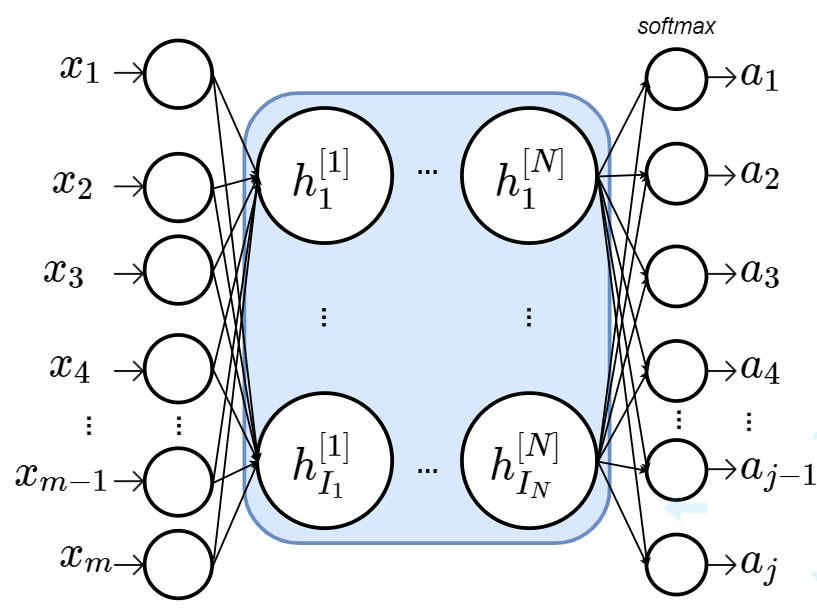
\includegraphics[width=8cm, keepaspectratio]{SimpleNN}
\caption{Simple neural network depicting $m$ inputs, $j$ outputs  $N$  hidden layers and with $I$ neuron in layer.}
\label{fig:SimplNN}

\end{figure}



%For professor: Should i insert activation function formula for each of the mentioned functions?

Before a neural network can be deployed, it needs to be trained to model non-linear high dimensional functions. The training of a neural network involves selecting the exact set of parameters, weights, biases and inactivation function that meet its specified objective. There are several algorithms that can tackle this non-linear optimization problem. A training dataset is a dataset of sample inputs which has  known outputs or labels. In supervised learning,  we feed the inputs from a training dataset to the neural network during its training phase and compare computed output with the corresponding labels.

Some of the most popular algorithms deployed in the training phase are variants of gradient descent (GD)  algorithm. In simple terms, the GD algorithm calculates the derivative of the function being optimized with respect to each of the current parameters. It then updates the parameters and repeats the process iteratively to achieve more accuracy. 
Gradients in Deep network are computed after both the feed forward and back propagation steps. In forward propagation, the inputs from a training set are passed to the network and its output is recorded. We then compare the computed output and provided labels to calculate the error or loss function. The error function is given by the difference between the label of the training set and the computed output by the neural network. The backpropagation algorithm then finds the partial derivative of the error function with respect to each neuron. This highlights how each neuron has contributed to the total error. We then use each neuron's computed error contribution and its corresponding activation value to calculate gradient. The parameters in the network are then adjusted to reduce the computed gradient.
 repeat these steps of forward pass, error calculation, back propagation and parameter update iteratively until the desired objective function is achieved.



%---------------------------------------------------------------------------------
\section{Background on Stochastic Gradient Descent}
%--------------------------------------------------------------------------------- 
Gradient Descent (GD) is an iterative algorithm that is often used to calculate the parameters of neural
networks, i.e., their weights and biases. At each iteration, the  algorithm updates the parameters based on the gradient of the 
an error function evaluated with the current parameters. The iterations continue until a minimum is reached. Since the objective
function is non-linear, the algorithm can only guarantee that it converges to a local minimum.

Explain how samples are used in GD....
Although GD is effective at finding the parameters of DNNs, it employs all the samples in the data set before updating the parameters,
which is computationally intensive and time consuming. To overcome this challenge, Stochastic Gradient Descent(SGD) has been
proposed. Unlike GD where all samples in the data set are used in a single iteration, SGD only selects a random subset
of samples for calculating the gradient and updating the parameters at each iteration. Since SGD only uses a fraction of the training
data set during each iteration, its computing time is significantly smaller compared to GD. Moreover, SGD is able to avoid local minima
because it search different parts of the solution space by randomly selecting samples at each iteration. 

%However, using a the path to local the minimum is
%noisier (WHAT DO YOU MEAN BY NOISIER?) than GD.
% However, the stochastic GD significantly reduces the training time of the network
%DO WE ACHIVE THE SAME RESULTS? IF NOT WHAT IS THE TRADE-OFF?

The size of the subset of samples, called mini-batch, used at each iteration has to be chosen carefully. A small batch can reduce the
computing time at each iteration, but may increase the number of iterations needed to converge. 
%The most popular gradient descent
%algorithm, however, is mini-batch Gradient Descent. This algorithm uses more than 1 sample for calculating gradient descent at each
%iteration and then the model is updated based on smaller groups of samples. 

%Mini-batch
%SGD converges in fewer iterations than GD whi


Formally, the SGD can is defined as follows. EXPLAIN HOW THE SAMPLES ARE CHOSEN. EXPLAIN THE ITERATIONS. 
SGD first initializes...

At each iteration, SGD...
Let $w$ denote the flattened
vector of all weights and biases of a deep neural
network. Let $E$ be an error function which is defined as the difference between the actual output of the objective function and the
predicted output of the network. 
%Our aim is to compute the slope of the cost function and the direction we should move to update our
%parameters. 
Then the $j$th parameter of $w$ is give by:
%\begin{equation*}
 $$w_j = w_j -\alpha \frac{\partial E_i}{\partial w_j}, $$
%\end{equation*}
where $\alpha$ is the learning rate,  $E_i$ is the value of the error function computed over minibatch $i$, and  
$\frac{\partial E_i}{\partial w_j}$ denotes the partial derivative of $E_i$ and $w_j$. 
 

%---------------------------------------------------------------------------------
\section{Problem Formulation}
%---------------------------------------------------------------------------------
In this section, we describe our considered collaborative deep learning model, and the threat model. 

%---------------------------------------------------------------------------------
\subsection{System Model} \label{sec:systemModel}
%---------------------------------------------------------------------------------
In this section, we describe a deep learning system with a pool of multiple participants. Each of the participant in this system has a
local private dataset available for training. We assume a reference participant such that the local private dataset of the reference
participant is significantly smaller when compared with other participants. All participants in this system agree in advance on a
common network architecture and common learning objective. The system also includes a secure parameter server (PS), which maintains the
latest values of parameters. 

%We consider a user who trains a deep neural network using his local data. However, as the user's local data is limited, it needs to
%collaborate with other users who have additional data to improve its own deep neural network. To this end, the user collects parameters
%from the other users ... [EXPLAIN HOW THE SYSTEM WORKS]

%--------------------------------------------------------------------------------------------
\section{System Architecture}
%--------------------------------------------------------------------------------------------

SEPARATE THE CONCEPTUAL ARCH FROM THE CODE

For this experiment, we implement a similar neural network structure for the reference user as well as other participants. It is a
multilayer perceptron (MLP) in a classic feed forward arrangement. We utilize the \textit{nn.Sequential} container via Torch nn package
to attach all the layers in a fully connected and feed forward manner. Each neural network is designed to have 1024 inputs
corresponding to each pixel in the provided 32x 32 pixel image of a handwritten number \cite{deng2012mnist}. The output layer is a
tensor of size 10 where each output corresponds to the probability that the given input is a specific number between 0 and 9. The model
also has 2 hidden layers where an activation function is applied to the output of each hidden layer.
Initially, the input is reshaped into a 1 dimensional tensor of size 1024 and funneled to the first hidden layer. The hidden layers are constructed via \textit{nn.Linear()} via which linear transformation can be applied. It then produces a tensor of size 128 as its output. The second hidden layer accepts a tensor of size 128 as input to yield a tensor of size 64 as output. We use a non-linear activation function called Rectified Linear Unit (ReLU) which is applied after each hidden layer. The last layer of the model is a log soft max layer coded by the \textit{nn.LogSoftMax()} module.  This activation function is usually applied to the end of all classification models where it squashes the inputs into probabilities that sum to one.
The Architecture described above are represented in Figure\ref{fig:MLPArch} as printed out by Torch7
   
The parameter server is responsible for maintaining the current values of all parameters. Since it should be accessible to all
participants , the server can be implemented as any form of updatable cloud storage. However, for the purpose of this experiment we
chose to implement it as another neural network. 

%--------------------------------------------------------------------------------------------
\subsection{Hyperparameter Setup}

%--------------------------------------------------------------------------------------------
Hyperparameters are parameters that control the collaborative learning process. Unlike the actual neural-network parameters, they are usually set before the training commences and remain unchanged during the process.
They are crucial since they directly influence the behavior of training algorithm and have a large impact on the performance and accuracy o the model.
The learning rate is set at $0.1$ and weight decay is set to $1e-7$. The batch size is 10 samples and the number of participants is 20. We vary the $\theta_u$ and epochs in different scenarios. 

\begin{figure}[!h]
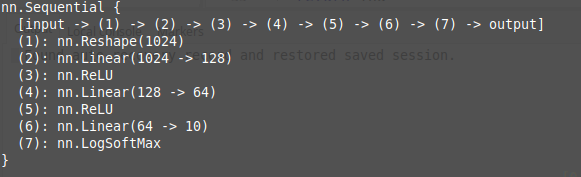
\includegraphics[width=8cm, keepaspectratio]{MLPArchitecture}
\caption{MLP architecture used for MNIST related experiments, as printed ou by Torch}
\label{fig:MLPArch}

\end{figure}

%---------------------------------------------------------------------------------
\subsection{Threat Model}
%---------------------------------------------------------------------------------

We consider a malicious collaborator who instead of sharing the parameters of its deep neural
network as described above, it collects the parameters from the target user to replicate its data, and ultimately violating the user's
privacy.  
Since the threat is not{} dependent on the adversary compromising the
central Parameter Server, it remains viable. In effect, the adversary does not have to control the parameter server or the service
provider to execute his attack. The attack is more effective when adversarial influence is exercised \cite{hitaj2017deep}. This would
imply that
the adversary is an active participant that is adapting his gradients in real time during the current learning process.

%describe an attack that results in privacy leakage in
%collaborative deep learning system proposed in
%\cite{Shokri}.  The attack results in a malicious user inferring sensitive information from a victim's dataset. 

%Specifically, the proposed attack the goal of the  adversary is to extract information from a victim about a class of data he does
%not own. The
%adversary deceives victim into releasing more information about the specific class by presenting himself as an honest participant in
%the collaborative learning  process.    The adversary does launches the
%attack by pretending to be an honest participant and building a local GAN unbeknownst to the other participants.

%The threat model is dependent on an active insider. However, 

%\subsection{Attack Posed}

In particular the attack operates as follows. Suppose all participants including the adversary agree on general specifications such as
the type of neural network and labels on which training would take place as described in Section \ref{sec:systemModel}. Let another
participant in the collaborative deep learning
model be the victim $V$ that declares the labels $[a,b]$. The adversary declares labels $[b,c]$ implying that the adversary has no data
on class $a$. By deploying the attack, the adversary stands to gain useful information about class a.

The adversary then uses the private GAN to generate models that look like class $a$, which the adversary deceivingly mislabels as $c$.
This prompts the victim  $V$ to release more information about the class $a$ in order to distinguish between classes 
$a$ and $c$. Therefore the victim releases more data on class a now than he initially intended to.

This can be further summarized as follows:
\begin {enumerate}
\item Assuming victim $V$ declares labels $[a,b]$ and adversary $A$ declares labels $[b,c]$
\item We then run the collaborative learning protocol for several epoch and stop when we reach a specified accuracy.
\item During this process, the $V$ downloads a percentage of parameters from parameter Server and updates his local model.
\item $V$'s local model is trained on classes $a$ and $b$
\item $V$ uploads a section of his model to Parameter Server
\item The adversary trains is slotted to engage with the Parameter Server
\item $A$ downloads the percentage of parameters from the PS and updates his model
\item $A$ then trains his local GAN to mimic class $a$.
\item $A$ generates class a samples from the GAN and mislabels them intentionally as class c.
\item $A$ uploads a percentage of his parameters to the PS
\end {enumerate}
During the process of convergence, $A$ will be able to covertly exert influence on the learning process via the mislabeling of class
$a$.

In this paper, we present a collaborative learning scenario that prevents the reference user from releasing more
information about a class, and ultimately it protects the reference user's privacy. We design the interaction of the reference user
with Parameter Server such that $V$ is not RefU

\section{A Privacy-preserving Collaborative Learning Algorithm}

The proposed system is designed to consider the reference participant with a much smaller data set as the most significant benefactor
of this privacy preserving deep learning architecture. We thereby structure the system to ensure that the privacy of the reference user
is not affected by the inventive GAN based attack proposed in \cite{hitaj2017deep}. Table 1 summarises the notations used in this paper


\begin{table}[!h]
\centering
\caption{Table1: Summary of notations used in the paper}
\label{table:1}
\begin{tabular}{ | m{0.12\columnwidth} | m{0.8\columnwidth}| } 
\hline
\textbf{Notation} & \textbf{Description} \\
 \hline\hline

N & Number of participants excpet the Reference User in the system\\
\hline
Reference User & The  main benefactor of the architecture \\
\hline
$M$ & Mini batch size used for stochastic gradient descent\\
\hline
$\theta_d$, $\theta_u$ & Fraction of parameters selected for download and upload from total available parameters \\
\hline
$W_k$ & Weight matrix for layer K in the neural network\\
\hline
$w$ & Flattened vector of all parameters in the neural network. \\
\hline
$\Delta w$ & Vector of changes in all local parameters due to SGD\\
\hline
$w^{(global)}$ & Flattened parameter vector for server\\
\hline
$E$ & Error Function defining the difference btween the computed value and expected value of the objective function \\
\hline
$\alpha$ & Learning rate of the stochastic gradient descent algorithm\\
\hline
$S$ & Set of $\theta_u$ largest indices selected from $w$ \\
\hline
\end{tabular}
\end{table}

%-------------------------------------------------------------------------------
\section{Experimental Setup}
%-------------------------------------------------------------------------------

We evaluate the learning performance of the reference user under our proposed privacy-preserving collaborative learning algorithm. We
measure ... and compare it to a the learning performance of a traditional deep neural network without collaborative learning. 
%We wrote the source code based on the pseudocode provided in paper \cite{Shokri}. 
We implement all algorithms using Torch with the neural network packages in the scripting language LUAJIT, and run them 
%We were able to replicate their original setup using
%Torch and nn packages in LUAJIT scripting language.  
%The tests on the proposed solution were run and hosted 
on an M4 instance on the Amazon Web Service's Elastic Compute Cloud (AWS EC2).

We used the MLP implementation of neural network using the function \textit{nn.Sequential} container via the Torch nn package. They are
fully connected and the neural network has input data of size 1024 (32 x 32) and feed fowards

%-------------------------------------------------------------------------------
\subsection{Datasets}
%-------------------------------------------------------------------------------
We conducted our experiments using the MNIST dataset \cite{deng2012mnist}. The MNIST dataset is a standard dataset used in image
recognition.
It contains images of hand-written grayscale digits ranging from 0 to 9. The dimension of each image is 32 X 32 pixels. There
are 60,000 such images in their training dataset and 10,000 images in their test dataset.

For this experiment, we normalize the images so that they are centered. 

We set the size of the local dataset of each participant to 1 \% of the training dataset images. 
The Reference User starts with a training set of 60 images.

%--------------------------------------------------------------------------------------------
%\subsection{Framework}
%---------------------------------------------------------------------------------------------

%We conduct our experiment within the Torch 7 and Torch 7 nn framework. Torch is a popular framework utilized for deep learning by major
%software companies. The code for the experiment is written in LuaJIT which is a scripting language based on Lua.  We deploy our
%architectural framework with multiple neural networks on the AWS EC-2 machine to leverage greater processing speed.


\section{Experiment Results}

\section{Conclusion}


\section{Authors and Affiliations}


\section{Identify the Headings}


\section{Figures and Tables}



\bibliographystyle{IEEEtran}
\bibliography{references}


\end{document}
